\documentclass[tikz, convert=pdf2svg]{standalone}

\usetikzlibrary{positioning, backgrounds, calc}
\begin{document}
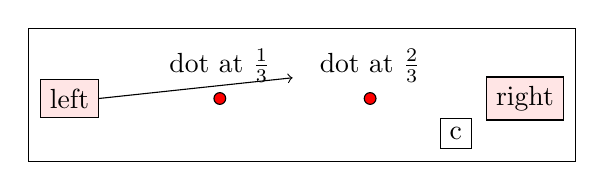
\begin{tikzpicture}[framed]
    \node[draw, fill=red!10] (left) {left};
    \node[draw, fill=red!10, right=140pt of left] (right) {right};
 
    \node[draw, inner sep=1.5pt, circle, fill=red, label={dot at $\frac{1}{3}$}] at ($(left)!0.33!(right)$) {};
    \node[draw, inner sep=1.5pt, circle, fill=red, label={dot at $\frac{2}{3}$}] at ($(left)!0.66!(right)$) {};

 \draw[->] (left.east) -- ($(left.north east)!0.5!(right.north west)$);
    \path let                          
        \p1 = (left.south),  
        \p2 = ($(left.east)!0.8!(right.north)$),     
        in node[draw, anchor=north west] (c) at (\x2,\y1) {c};
\end{tikzpicture}
\end{document}
